\documentclass[12pt]{article}

\usepackage[utf8]{inputenc}
\usepackage[brazil]{babel}
\usepackage[a4paper,left=3cm, right=2cm,top=2.5cm, bottom=2.5cm]{geometry}
\usepackage{amsmath}
\usepackage{graphicx}
\usepackage{float}
\usepackage{multirow}
\usepackage{authblk}
\usepackage{fancyhdr}
\usepackage{xcolor}
\usepackage{cite}


\title{\textbf{ENG1456 - Algoritmos Genéticos - Trabalho 1}}
\author{\textbf{Aluno: Matheus Carneiro Nogueira - 1810764}}
\affil{}
\author{\textbf{Professora: Karla Figueiredo}}
\affil{}
\pagestyle{fancy}
\fancyhf{}
\lhead{{\small \textcolor{gray}{PUC-Rio ENG1456}}}
\renewcommand{\headrulewidth}{0pt}
\date{}
\renewcommand{\footrulewidth}{0pt}
\fancyfoot[C]{\thepage}

\begin{document}
	\maketitle
	\tableofcontents
	
	
	\begin{abstract}
		Este documento consiste no relatório do trabalho 1 do módulo de Algoritmos Genéticos da disciplina ENG1456 da PUC-Rio. O objetivo deste trabalho é estudar diferentes modelos de Algoritmos Genéticos para a tentativa de otimização da função $F6$ apresentada em sala. Foi utilizado o programa \textit{GADEMO} para gerar os modelos pedidos nos enunciados. Em todas as figuras do GADEMO em que há mais de uma curva plotada, as configurações são referentes apenas à última curva. Foram consultados os materiais de aula, o livro \cite{davis1991handbook} e outros materiais devidamente referenciados.
	\end{abstract}
	
\section{Reproduzindo Resultados}

\textbf{Enunciado:}
Variando os parâmetros, execute Algoritmos Genéticos de modo a obter resultados semelhantes aos apresentados no livro texto. Os parâmetros usados no livro se encontram na tabela abaixo. Compare as curvas referentes à média de 20 rodadas de cada GA. Incluir dois gráficos: um com GA1-1, GA2-1 e GA2-2 e outro com GA 2 -3 e GA2-4. Utilizar somente one-point-crossover.

\begin{figure}[H]
	\centering
	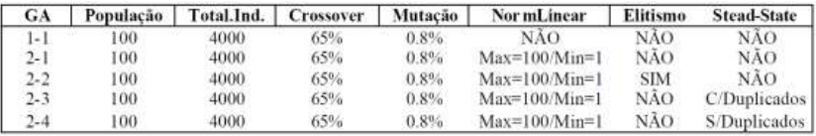
\includegraphics[width=0.9\linewidth]{Imagens/tabela_especificacao_modelos}
	\caption{Tabela com as especificações dos modelos}
	\label{fig:tabelaespecificacaomodelos}
\end{figure}


As duas imagens abaixo exibem os 5 GA's solicitados no enunciado. Em ambas as figuras também foi plotada a curva da busca aleatória para fins de comparação.

\begin{figure}[H]
	\centering
	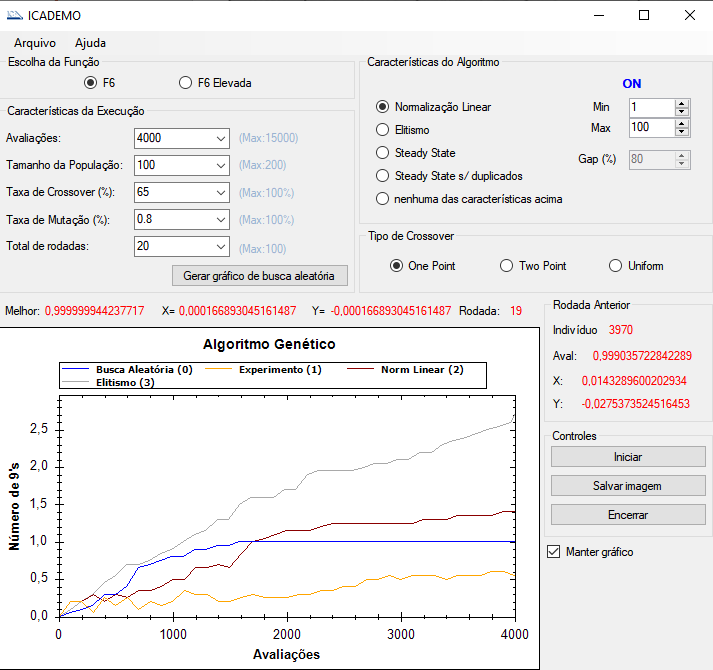
\includegraphics[width=0.7\linewidth]{Imagens/questao1_1}
	\caption{Experimento 1: GA=1-1, Norm. Linear: GA=2-1, Elitismo: GA=2-2}
	\label{fig:questao11}
\end{figure}

\begin{figure}[H]
	\centering
	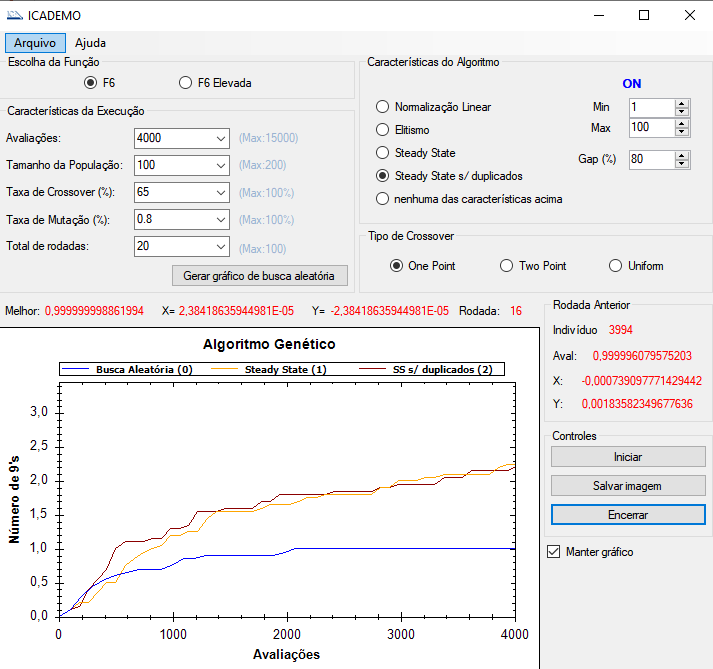
\includegraphics[width=0.7\linewidth]{Imagens/questao1_2}
	\caption{Steady State 1: GA=2-3, SS s/ duplicados: GA=2-4}
	\label{fig:questao12}
\end{figure}

Podemos, facilmente, perceber alguns detalhes imporantes. Primeiramente, o GA 1-1 da figura \ref{fig:questao11} se mostrou pior que a busca aleatória. Isso não é surpresa,  uma vez que esse modelo não usufrui de nenhum operador além do crossover e mutação. Ao analisar as demais curvas que utilizam esses recursos, é de se esperar que o resultado seja melhor que uma busca aleatória, senão não haveria motivo para utilizar um algoritmo genético.

Uma simples normalização linear já foi suficiente para que o GA 2-1 apresentasse melhor resultado que a busca aleatória.

A utilização do elitismo é importante por garantir que, durante a evolução, o melhor indivíduo de $t+1$ seja sempre melhor ou igual ao melhor de $t$. Isso se percebe pelo fato da curva cinza da figura \ref{fig:questao11} ser monotônica, isto é, sempre crescente. Esse fato é suficiente para explicar o melhor desempenho desse modelo em relação aos anteriores.

Ambos os Steady States foram utilizados com GAP=80\%, o que quer dizer que 80\% dos indivíduos de uma geração serão trocados para a próxima geração e os melhores 20\% serão mantidos. A análise do GAP ideal será realizada na seção seguinte. A opção sem duplicados quer dizer que, a cada geração, será verificado se algum filho gerado é igual a algum indivíduo da parte que foi mantida e, se for, um novo filho será gerado. Isso, em teoria, aumenta a diversidade da população.

Comparando as duas figuras, podemos perceber que, dentre os 5 GA's apresentados e a busca aleatória, aquele que utiliza elitismo junto com normalização linear (GA2-2) apresenta o melhor resultado.

\section{GAP ideal}
\textbf{Enunciado:} Para os GAs que utilizam steady-state, determine o GAP (número de indivíduos substituídos a cada ciclo) ideal. Para isso, use um incremento de 5 indivíduos a cada tentativa, começando com um GAP=5. Não entregue os gráficos referentes aos testes de GAP.\\

O melhor resultado para cada GAP é exibido nas tabelas as seguir.

\begin{table}[H]
	\centering
	\begin{tabular}{|c|c|c|c|c|c|c|c|c|}
		\hline
		GAP & 5 & 10 & 15 & 20 & 25 & 30 & 35 & 40 \\
		\hline
		Num de 9's &2.6  &2.1  &2.5  &2.5  &3.4  &2.3  &2.45  &2.5  \\
		\hline
		GAP & 45 & 50 & 55 & 60 & 65 & 70 & 75 & 80 \\
		\hline
		Num de 9's &2.25  &2.2  &3.7  &3.5  &1.95  &2.0  &2.6  &3.05  \\
		\hline
		GAP & 85 & 90 & 95 & 100 &  &  &  &  \\
		\hline
		Num de 9's &2.6  &2.9  &2.85  &1.75  &  &  &  &  \\
		\hline
	\end{tabular}
	\caption{Tabela com melhor resultado para cada GAP Steady State com duplicados}
\end{table}

\begin{table}[H]
	\centering
	\begin{tabular}{|c|c|c|c|c|c|c|c|c|}
		\hline
		GAP & 5 & 10 & 15 & 20 & 25 & 30 & 35 & 40 \\
		\hline
		Num de 9's &3.0  &2.2  &3.15  &2.85  &3.45  &3.7  &3.45  &3.15  \\
		\hline
		GAP & 45 & 50 & 55 & 60 & 65 & 70 & 75 & 80 \\
		\hline
		Num de 9's &1.9  &2.3  &2.0  &2.4  &2.1 &3.0  &3.55  &4.35  \\
		\hline
		GAP & 85 & 90 & 95 & 100 &  &  &  &  \\
		\hline
		Num de 9's &3.9  &2.6  &1.9  &1.6  &  &  &  &  \\
		\hline
	\end{tabular}
	\caption{Tabela com melhor resultado para cada GAP Steady State sem duplicados}
\end{table}

\begin{figure}[H]
	\centering
	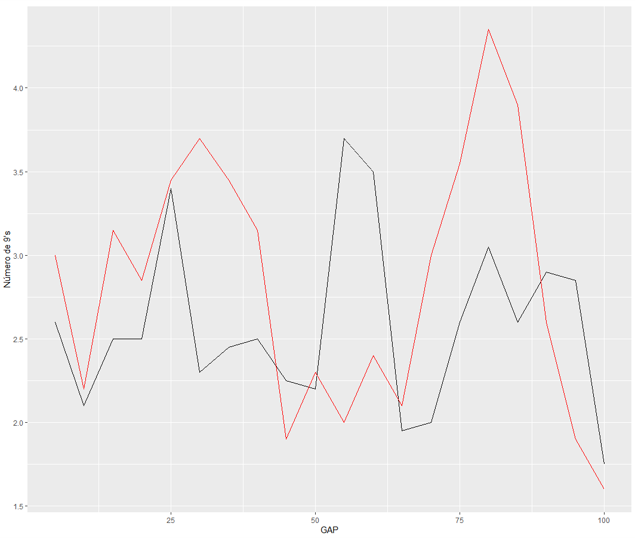
\includegraphics[width=0.7\linewidth]{Imagens/comparacaoGAP}
	\caption{Linha preta = Com Duplicados; Linha vermelha = Sem Duplicados}
	\label{fig:comparacaogap}
\end{figure}


Como explicado na seção anterior, GAP significa a porcentagem da população que será trocada. Logo, um GAP de 0\% significaria que nenhuma parcela da população seria trocada, ou seja, a evolução ficaria congelada. Por outro lado, um GAP de 100\% seria equivalente a não haver Steady State. Sendo assim é necessário um equilíbrio entre o número de indivíduos mantidos e trocados. Se mantivermos indivíduos demais, a evolução pode se tornar lenta e estagnada, pois haverá pouca geração de novos indivíduos. Caso contrário, vamos regredir ao modelo sem Steady State, pois nenhum indivíduo será mantido e teremos a geração normal de filhos.

Como imaginado, os melhores resultados não são os valores limites do GAP, como visto na \ref{fig:comparacaogap}. No entanto, percebe-se uma evolução distinta entre os casos com e sem duplicados. Para o primeiro, os melhores valores foram próximos de 80\%, enquanto para o caso sem duplicado, próximo de 55\%. Podemos notar que, para GAP de 100\%, ambos os modelos apresentam melhor valor próximo do melhor valor do modelo apenas com normalização linear, o que também era esperado.

Conclusões acerca da evolução da qualidade com o aumento do GAP e do perfil de cada curva da figura \ref{fig:comparacaogap} mais aprofundadas eu sou incapaz de realizar.
	
\section{Taxas Crossover e Mutação}
\textbf{Enunciado:}
Verifique o que acontece quando se roda o GA2-1 20 vezes com taxa de crossover muito baixa (pouca recombinação em torno de 10\%) e alta taxa de mutação (muitas mudanças aleatórias em torno de 80\%). Imprima o resultado (um gráfico), compare com o resultado do GA2-1 obtido no item 1 e explique
brevemente o que acontece.\\

A figura \ref{fig:questao3} abaixo exibe o GA com as taxas pedidas.

Sabemos que a altas taxas de mutação aumentam a aleatoriedade do processo de evolução e que baixas taxas de crossover tornam a busca pela seleção ótima mais lenta, uma vez que há menor combinação dos progenitores.

Ao analisar a figura \ref{fig:questao3} podemos perceber uma alta volatilidade na qualidade da solução, isto é, grnade variação entre picos e vales. Esse fato é resultado da alta taxa de mutação, uma vez que ela atrapalha a evolução normal do algoritmo ao adicionar aleatoriedade. A baixa taxa de mutação, por sua vez, é percebida de forma mais sutil pela falta de caráter crescente da curva. Como são feitos poucos cruzamentos, utiliza-se pouco os bons progenitores para gerar bons filhos, o que diminui a qulidade da evolução da solução. 

\begin{figure}[H]
	\centering
	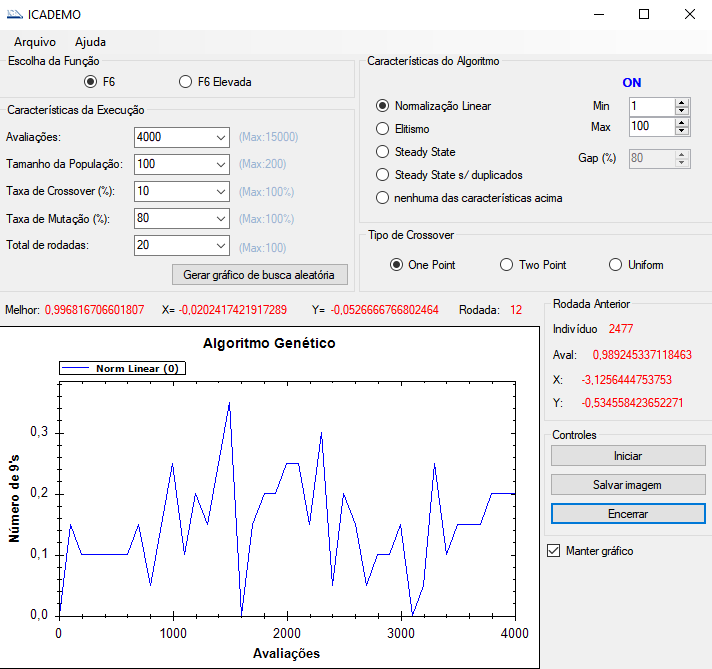
\includegraphics[width=0.7\linewidth]{Imagens/questao3}
	\caption{GA2-1 com taxas de crossover 10\% e mutação 80\%}
	\label{fig:questao3}
\end{figure}


\section{Tamanho da População}
\textbf{Enunciado:}
Analise o efeito do tamanho da população, obtendo as curvas de desempenho do GA2-2 (20 rodadas) para vários tamanhos de população (ex: 20, 50, 100, 150) e sempre com o mesmo número de gerações (total de indivíduos variável). Imprima as curvas para e tire conclusões sobre o efeito do tamanho da população no desempenho do
algoritmo genético.\\

Antes de partirmos para a avaliação dos diferentes GA's, devemos lembrar como definir o tamanho da população em relação do número de gerações e do número total de indivíduos(avaliações).

Esses parâmetros relacionam-se de acordo com a seguinte expressão:

\begin{equation*}
	avaliacoes=num\_geracoes\times tamanho\_populacao
\end{equation*}

A partir dessa relação e dos valores solicitados pelo enuncido para os tamanhos de população, mantendo o número de gerações igual a 40, chegamos aos seguintes valores:

\begin{table}[H]
	\centering
	\begin{tabular}{|c|c|c|c|c|}
		\hline
		tam\_pop & 20 & 50 & 100 & 150 \\
		\hline
		avaliações & 800 & 2000 & 4000 & 6000 \\
		\hline
	\end{tabular}
\end{table}

A figura abaixo exibe os resultados para esses valores de população.

\begin{figure}[H]
	\centering
	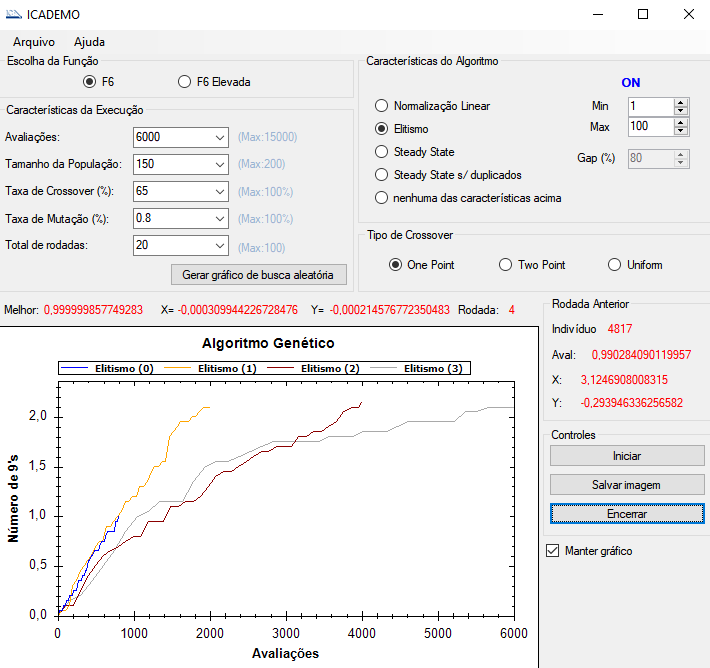
\includegraphics[width=0.7\linewidth]{Imagens/questao4}
	\caption{Elitismo (0) = tam\_pop=20; Elitismo (1) = tam\_pop=50; Elitismo (2) = tam\_pop=100; Elitismo (3) = tam\_pop=150;}
	\label{fig:questao4}
\end{figure}

Podemos, a partir da análise da imagem, concluir que uma população de 20 indivíduos com 40 gerações é pouco para a evolução do algoritmo. O que nos indicar esse fato é a curva amarela da figura \ref{fig:questao4}, que representa a população de 50, ser praticamente a mesma da curva azul, população de 20, até o número de avaliações existentes na curva azul. Isso nos indica que, se houver mais do que 20 indivíduos por população, o algoritmo seria capaz de evoluir mais em direção à solução ótima. 

Por outro lado, para as populações de 50, 100 e 150, o resultado final da soluçao é muito similar, ficando em torno de 2.1 noves. Isso nos revela que aumentar o número de indivíduos da população mantendo a mesma quantidade de gerações não infere, necessariamente, na melhora da solução. Podemos justificar isso da seguinte maneira: mais indivíduos por população aumenta o paralelismo da busca, mas, em dado momento, o algoritmo já possui indivíduos suficientes buscando a solução ótima e precisaria, apenas, de mais tempo (gerações) para encontrá-la. 

\section{Convergência}
\textbf{Enunciado:}
Repita o GA2-1 e o GA2-2 (20 rodadas cada) modificando apenas o total de indivíduos criados para o 10000. Imprima as curvas em dois um gráficos separados, um para o GA2-1 e outro para o GA2-2, e verifique se é vantajoso todo esse esforço computacional, em outras palavras, determine o número de
indivíduos para o qual cada algoritmo converge.

A figura abaixo exibe os resultados dos GA's solicitados no enunciado.

\begin{figure}[H]
	\centering
	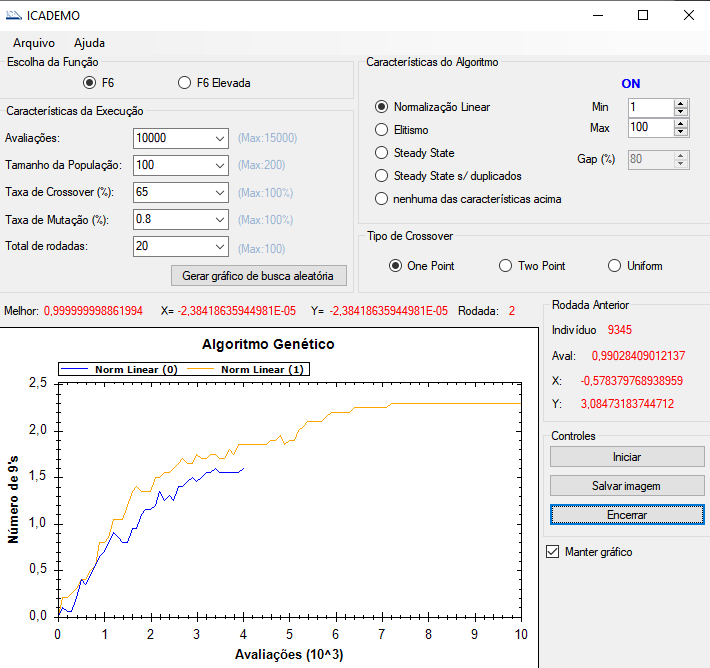
\includegraphics[width=0.7\linewidth]{Imagens/questao5_1}
	\caption{GA 2-1 com avaliações de 4000 (azul) e 10000 (amarelo)}
	\label{fig:questao51}
\end{figure}

\begin{figure}[H]
	\centering
	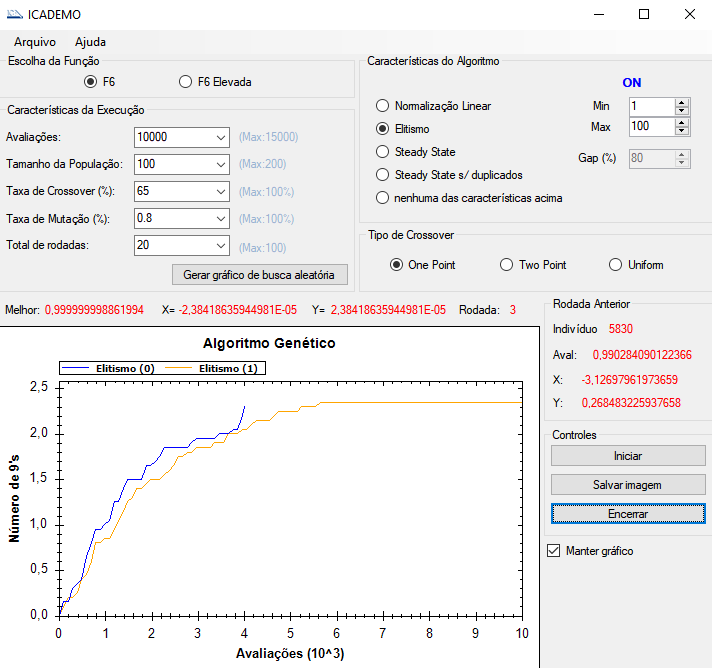
\includegraphics[width=0.7\linewidth]{Imagens/questao5_2}
	\caption{GA 2-2 com avaliações de 4000 (azul) e 10000 (amarelo)}
	\label{fig:questao52}
\end{figure}

A análise de convergência dos GA's fornece conclusões distintas para o caso com e sem elitismo. Comecemos pelo GA 2-1, com normalização linear e sem elitismo.

Nesse caso, percebe-se pela figura \ref{fig:questao51} que não há uma convergência para o mesmo valor de avaliação, isto é, o algoritmo com mais avaliações (curva amarela) apresentou um desempenho melhor que o com menos (curva azul). Isso pode ser explicado pelo fato de, em elitismo, não garantirmos que a curva de avaliação será sempre crescente. Sendo assim, precisamos de mais tempo, ou seja, mais avaliações e gerações, para chegar a um resultado mais próximo do ótimo, o que é evidenciado pela diferença entre as curvas.

Para o GA 2-2, com elitismo e normalização linear, a conclusão é outra. Com a utilização do elitismo, percebemos convergência para o mesmo valor de número de noves. Note que a curva amarela, após alcançar o valor mais alto da curva azul (2.6), permanece praticamente constante. Com esse operador, geramos uma curva monotônica e convergimos para um valor bom mais rapidamente. Isso nos mostra que aumentar a população de um GA com elitsmo não gera melhores resultados, uma vez que esse operador já é suficiente para produzir uma solução boa. Aumentar o esforço computacional, nesse caso, é desncessário e, dito isso, não recomendável.

\section{Crossover}
\textbf{Enunciado:}
Compare o efeito dos 3 tipos de crossover disponíveis na ferramenta, executando o GA2-1 (s/ elitismo) e o GA2-2 (c/elitismo) com apenas 2500 indivíduos (20 rodadas) para cada tipo de crossover, usando taxa de crossover 80\%. Imprima as curvas em dois um gráficos separados , um para o GA2-1 e outro para o GA2-2, e tire conclusões a respeito da característica conservadora/destrutiva de cada crossover.

As figuras abaixo exibem os gráficos para os 3 tipos de crossover para os GA's 2-1 e 2-2.

A grande diferença e, possivelmente, vantagem, dos crossovers de 2 pontos e uniforme é a maior capacidade de combinação entre os padrões dos genitores. Essa característica, por sua vez, aumenta a diversidade dos filhos gerados, uma vez que mais padrões podem ser construídos. No caso do GA com elitismo, figura \ref{fig:questao62}, pouca diferença é notada na evolução do algoritmo com os diferentes tipos de cruzamento. No entanto, os últimos indivíduos revelam um salto de qualidade para o crossover uniforme que não é percebido nos demais. É possível que esse bom desenvolvimento final possua relação com o tipo de crossover, mas a relação não é auto evidente.

Para o GA sem elitismo, mas apenas com normalização linear, o crossover uniforme foi, claramente, o pior operador entre os três. Isso se deve ao fato dele aumentar a recombinação de genes dos genitores o que, de certo modo, aumenta a aleatoriedade do processo de evolução que, sem o elitismo para garantir uma curva sempre crescente, mostra-se prejudicial para a evolução do problema. Os outros dois crossovers, de 1 e 2 pontos, fornecem resultados muito similares, mas com uma diferença, a opção de 2 pontos apresenta curva de evolução quase sempre crescente. Para averiguar se isso é devido ao crossover ou não, deveríamos treinar mais GA com essas características. Faremos isso na última seção.

\begin{figure}[H]
	\centering
	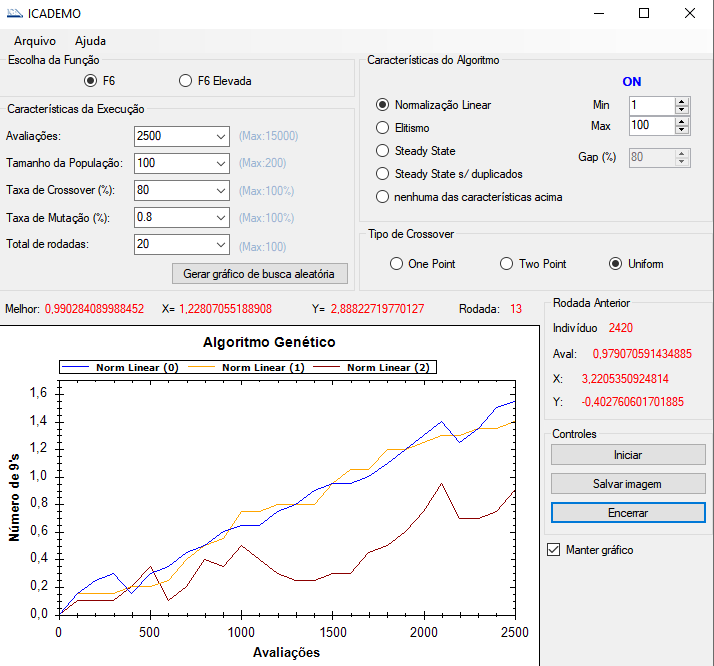
\includegraphics[width=0.7\linewidth]{Imagens/questao6_1}
	\caption{GA 2-1; Norm Linear (0) = crossover de um ponto ; Norm Linear (1) = crossover de dois pontos ; Norm Linear (2) = crossover uniforme}
	\label{fig:questao61}
\end{figure}
\begin{figure}[H]
	\centering
	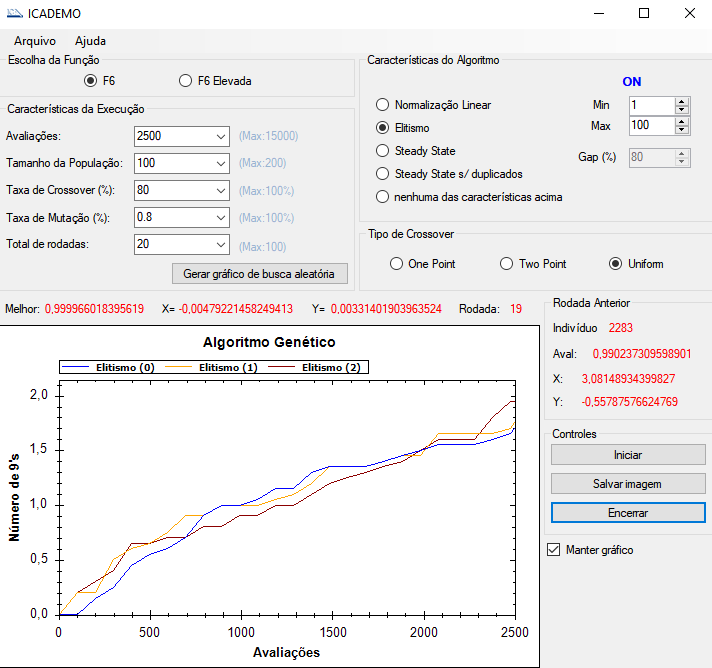
\includegraphics[width=0.7\linewidth]{Imagens/questao6_2}
	\caption{GA 2-2; Elitismo (0) = crossover de um ponto ; Elitismo (1) = crossover de dois pontos ; Elitismo (2) = crossover uniforme}
	\label{fig:questao62}
\end{figure}


\section{Normalização Linear}
\textbf{Enunciado:}
Repita o GA2-3COM gap = 75 para vários valores de máximo. Verifique o que acontece quando o valor de máximo aumenta e diminui (avalie para os valores 10, 50, 100, 200, 300). Imprima as curvas em apenas um gráfico e tire breves conclusões.\\

Sabemos que a normalização linear trabalha com aptidão $A_i$ definida como se segue:

\begin{equation*}
	A_i=min+\dfrac{max-min}{pop\_size-1}\times (i-1)
\end{equation*}

Dito isso, quanto maior o valor de \textit{máximo}, maior o valor dado à aptidão do indivíduo, o que, por sua vez, aumenta a pressão seletiva sobre os melhores indivíduos. É de se esperar, portanto, que tanto valores pequenos demais quanto grandes demais não se mostrem interessantes para fins de otimização, pois pouca pressão fará com que indivíduos ruins se reproduzam e pressão demais fará com que poucos indivíduos sejam selecionados para reprodução. A figura \ref{fig:questao7} exibe os resultados para valores de máximo de 10, 50, 100, 200, 300.

\begin{figure}[H]
	\centering
	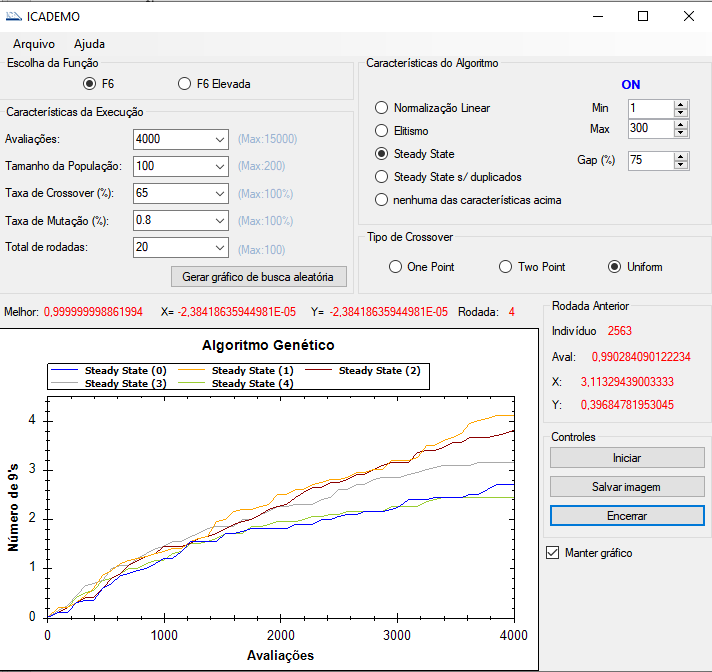
\includegraphics[width=0.7\linewidth]{Imagens/questao7}
	\caption{Steady State (0) = max 10; Steady State (1) = max 50; Steady State (2) = max 100; Steady State (3) = max 200; Steady State (4) = max 300;}
	\label{fig:questao7}
\end{figure}

Pela análise da figura, percebemos algo similar ao previsto. Os valores 10 e 300 para máximo, que são o menor e o maior de nossa lista de valores, apresentaram os piores resultados. O motivo é, justamente, o que foi comentado acima: pressão demais ou pressão de menos não é vantajoso para a evolução da solução, uma vez que o primeiro gera filhos inadequados e o último exerce pressão demais.  Seguindo esse raciocínio, é trivial entender porque os melhores valores de máximo, de acordo com a figura, foram os valores 50 e 100.

\section{Gerais}
\textbf{Enunciado:}
Fazendo variações nos parâmetros e técnicas disponíveis no GADEMO, estude livremente o efeito de cada umdestes no desempenho de algoritmos genéticos. Destaque e explique uma importante constatação.\\


\textbf{Novos testes com crossover de 2 pontos e GA 2-1}
O intuito desses testes é verificar se o comportamento quase monotônico da curva de avaliações apresentada para o GA 2-1 com crossover de 2 pontos é coincidência ou fruto dos parâmetros do algoritmo. A figura abaixo exibe os resultados.

\begin{figure}[H]
	\centering
	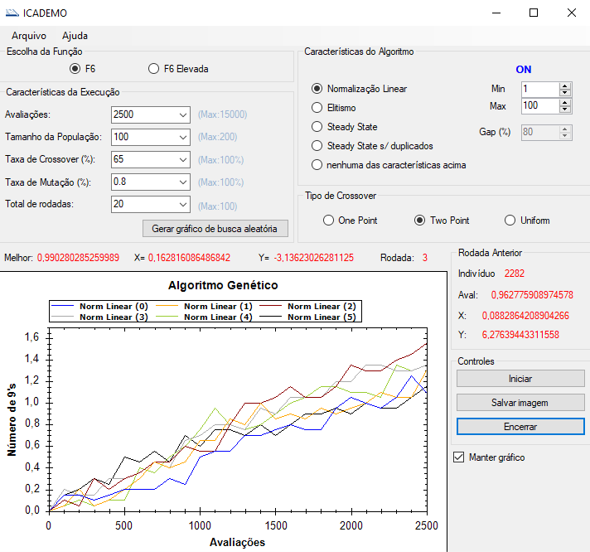
\includegraphics[width=0.7\linewidth]{Imagens/questao8_2pontos}
	\caption{GA 2-1 com crossover de 2 pontos}
	\label{fig:questao82pontos}
\end{figure}

Dada a figura \ref{fig:questao82pontos}, podemos perceber que o perfil monotônico anterior foi apenas fruto do acaso e uma especificidade daquele processo de evolução. Para outros 6 algoritmos com mesmos parâmetros, esse comportamento não foi observado.\\

\textbf{GAP = 1\%}

Anteriormente comentei que GAP's muito pequenos tornariam a evolução do algoritmo lenta e estagnada. Para verificar se isso, de fato, ocorre, foram gerados 6 GA's 2-3 com GAP=1\%, o menor valor possível no GADEMO. A imagem abaixo exibe os resultados.

\begin{figure}[H]
	\centering
	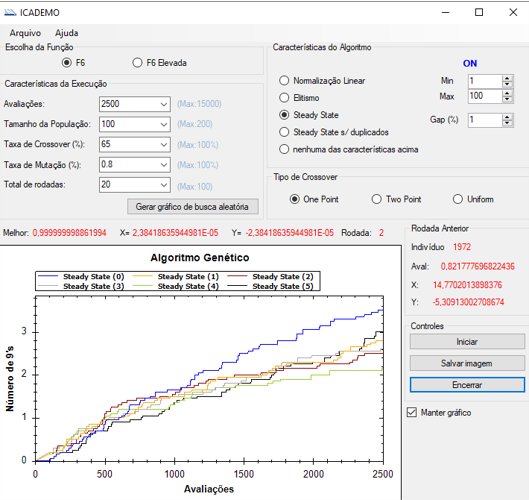
\includegraphics[width=0.7\linewidth]{Imagens/questao8_GAPpequeno}
	\caption{GA 2-3 com GAP=1\%}
	\label{fig:questao8GAPpequeno}
\end{figure}

Podemos notar que a suposição anterior não se mantém frente a esses resultados. Embora a evolução seja mais irregular, pois vemos vários degraus nas curvas da figura \ref{fig:questao8GAPpequeno}, ela é, obviamente, não constante e, na verdade, quase sempre crescente. A presença dos degraus pode ser explicada da seguinte maneira: com um GAP pequeno, muitos indivíduos são mantidos e apenas alguns novos são gerados. Com isso, as curvas apresentarão maiores porções horizontais, uma vez que de uma geração para outra pouca coisa será alterada.

	\bibliography{bibliografia} 
	\bibliographystyle{plain}
\end{document}